
%------------------------ HEADER ------------------------%

\documentclass{egpubl}
\usepackage{eurovis2016}

\STAR_Eurovis
\electronicVersion

\PrintedOrElectronic

\usepackage{t1enc}
\usepackage{dfadobe}
\usepackage[pdftex]{graphicx}
\usepackage{cite}
\usepackage{mathtools}



%------------------------ TITLE & AUTHOR ------------------------%

% \title[short title (shown on every page on top)]{full paper title}

\title[Seminar Report]{Procedural Modelling of Complex Systems}

% \author[short name (shown on every page on top]{full author name}

\author[B. Rainer \& S. Farda]
       {Bernhard Rainer$^{1}$ and Silvester Farda$^{1}$
        \\
         $^1$TU Wien, Austria}

\begin{document}


%------------------------ TEASER ------------------------%

\teaser{
  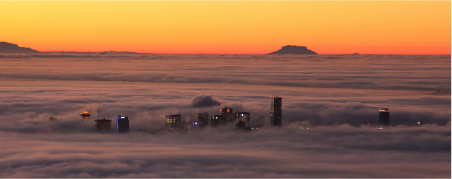
\includegraphics[width=\linewidth]{teaser}
  \centering
  \caption{Terrain generated from a river graph \cite{Genevaux:2013:TGU:2461912.2461996} and primitive features \cite{CGF:CGF12530}.}
  \label{fig:teaser}
}

\maketitle

\begin{abstract}
	Terrain modelling and representation is a elaborated topic in computer graphics and visualization. This report highlights some of the state-of-the-art techniques for large scale modelling of terrains, as well was modelling procedurally generation of content. We take a closer look on feature based modeling approach, where iconic landmarks, such as rivers or hills, can be combined with base terrain features to produce arbitrary, but realistic looking terrains. A large part in terrain generation is the creation of drainage networks and the influence of fluids to the terrain. We examine a procedure, that generates a functioning river network and create a terrain around it. Lastly the influence of water on terrain is a big research field. Here we look deeper into algorithms, that simulate the erosion of terrain due to fluid streams, accounting for both sediment and dissolve of soil material. 
	Also particle based calculation models are a very important topic in this field. Most of the utilized algorithms are purely physics-based have just been simplified to yield better results and/or to reduce it's computational demands. Due to some of those algorithms being quite complex, they go far beyond the scope of this report. Therefore it is our goal to present an overview of available techniques, rather than providing an exact and complete summary of the underlying publications.

	
	\begin{classification} % according to http://www.acm.org/about/class/2012
		\CCScat{Computing methodologies}{Computer graphics}{Rendering}
	\end{classification}
	
\end{abstract}



%------------------------ DOCUMENT ------------------------%
\input{Introduction}
\section{Terrain Modeling from Feature Primitives}
\label{sec:tmffp}
In \cite{CGF:CGF12530} a practical approach is described to model terrains using a construction tree, whose leave nodes are feature primitives. Such primitives describe landmark features, like rivers, mountains, valleys, lakes, and more universal features, like valleys, roughness, hills. The construction tree combines these primitives using a set of operators, which describe the type of combination. 

\subsection{Primitives}
A primitive can either be image based, or skeletal-based. Both primitives feature an elevation function and a weight function that describe the height of the terrain, as well as the potential interaction with other primitives. Skeletal-based primitives profit from a short render time and smaller memory footprint, whereas image-based primitives have a higher memory cost, but provide an easier way to integrate real data into the scene. 

\subsubsection{Skeletal primitives}
Skeletal primitives are defined by a geometric skeleton (point, segment, curve or contour) and a set of parameters that describe the elevation and the weight function. 

A \textbf{disc primitive} contains several parameters, such as the center c and radius r, describing the area of influence, as well as a noise function $\eta(p) $, which controls the local ground roughness. $\{a_i\}$ is a set of decreasing amplitudes, $\{s_i\}$ a set of increasing frequencies. Combining these parameter one can obtain the elevation function
\begin{center}
$ f(p) = c_{z} +  \sum\limits_{i = 0}^{n-1}(a_i\eta((p-c)s_i))$. 
\end{center}

\begin{figure}[htb]
	\centering
	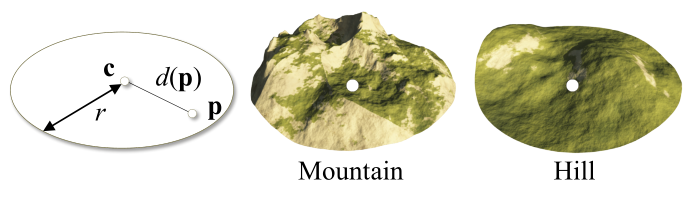
\includegraphics[width=.8\linewidth]{GGP15/disc_primitive}
	\caption{This figure shows a disc primitive creating a circular landform. The mountain is obtained using ridge-multifractal noise function, smooth hills are created using a turbulence function.}
	\label{fig:disc_primitive}
\end{figure}

\textbf{Curve primitives} are made up of a piecewise curve skeleton  $\Gamma$ and a set of profiles $\{c_i\}$. A profile describes a cross section perpendicular to the skeleton. Any function can be used to describe the cross section, in this example each cross section described as a one-dimensional quadratic function. The position is then constructed by interpolation using the curvilinear coordinates. 

One large use of curve primitives is rivers. A river follows its path, described with the curve skeleton. Using different profiles a homogenous shore can be obtained. More complex profiles can describe larger river systems like deltas and side streams. 
Modifying the profile accordingly, one can simulate roads with this model, by parametrizing the cross section with the road width and defining the elevation of the road in order to allow combination with other primitives in the terrain.

\begin{figure}[htb]
	\centering
	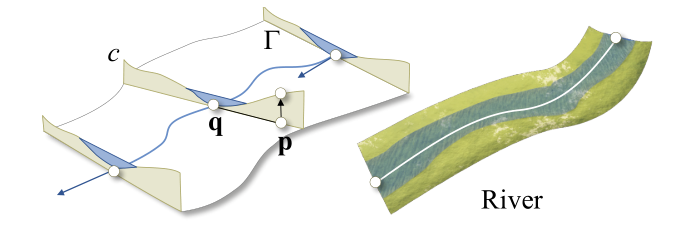
\includegraphics[width=.8\linewidth]{GGP15/curve_primitive}
	\caption{A curve primitive is used to create a river. $q$ corresponds to the projection of p onto the skeleton.}
	\label{fig:curve_primitive}
\end{figure}

\textbf{Contour primitives} describes a closed curve around a center point and a set of profile curves $\{ c_i \}$. Much like with curve primitives the profile curves describe the elevation in radial direction. This approach allows to compose more complex features.

\begin{figure}[htb]
	\centering
	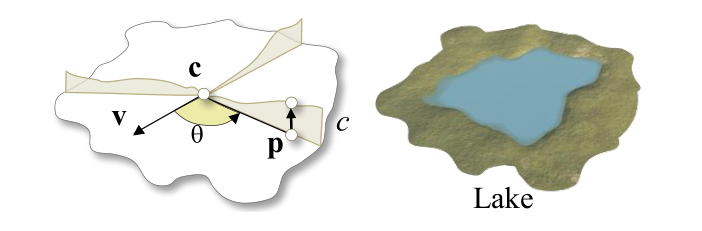
\includegraphics[width=.8\linewidth]{GGP15/contour_primitive}
	\caption{A contour polygon describes a complex system of polygons. In this figure it is used to describe a lake.}
	\label{fig:contour_primitive}
\end{figure}

\subsubsection{Image primitives}
Complex terrain features are difficult to create procedurally. To add complex feature, such as detailed river shores or sand ripples, image based primitives are used. This process is similar to using a heightfield on a terrain. 

\begin{figure}[htb]
	\centering
	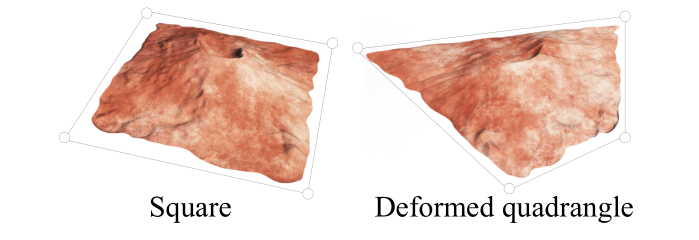
\includegraphics[width=.8\linewidth]{GGP15/image_primitive}
	\caption{Real data is mapped onto a quadrangle that can be deformed arbitrarily.}
	\label{fig:image_primitive}
\end{figure}


\subsection{Operators}
Much like in Constructive Solid Geometry the inner nodes of the construction tree are operators. These operators combine the elevation function $f$ and weight function $\alpha$ of their sub-trees. For simplicity we consider binary nodes and denote the two sub-trees $A$ and $B$. 

\subsubsection{Blending}
The elevations of two nodes are mixed according to their corresponding weight function. This allows to combine large scale terrain primitives in an effective matter. If two primitives are far away, they do not influence each other. The resulting terrain is the union of two sub-trees. If their regions of interest intersect they blend together.
\begin{figure}[htb]
	\centering
	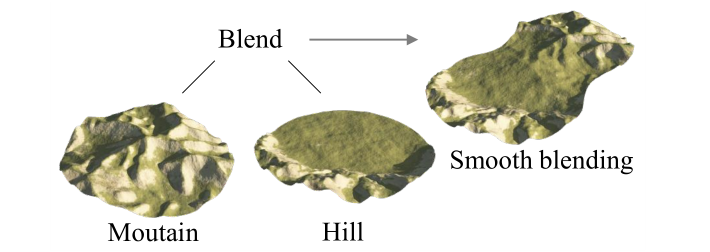
\includegraphics[width=.8\linewidth]{GGP15/blend_operator}
	\caption{This figure shows a blending of a mountain and hill to a smoother landscape. the areas of interest intersect partly. }
	\label{fig:blend_operator}
\end{figure}
\subsubsection{Replacement}
This operator defines specific local changes in the terrain. Such changes for example are lakes, rivers, roads. If the areas of interest intersect, the elevation in A is replaced with the value in B. 
\begin{figure}[htb]
	\centering
	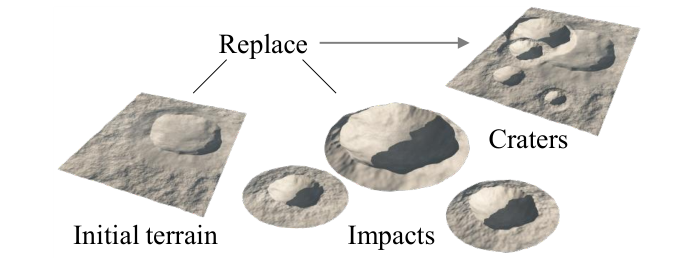
\includegraphics[width=.8\linewidth]{GGP15/replace_operator}
	\caption{Replacement is used to construct a lunar landscape..}
	\label{fig:replace_operator}
\end{figure}
\subsubsection{Addition}
The addition operator is used to add variations and details to the terrain. The additional elevation to $f_A$ is controlled by the product of $f_B$ and $\alpha_B$
\begin{figure}[htb]
	\centering
	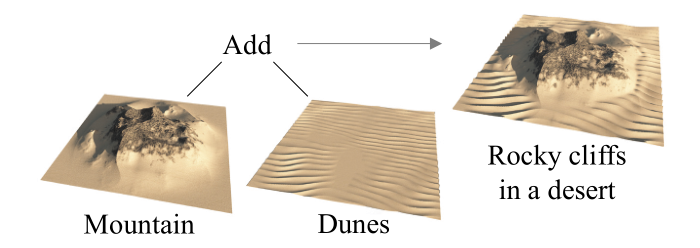
\includegraphics[width=.8\linewidth]{GGP15/addition_operator}
	\caption{Real data is mapped onto a quadrangle that can be deformed arbitrarily.}
	\label{fig:addition_operator}
\end{figure}
\subsubsection{Warping}
The warping operator allows to distort the shape of a surface by displacing the elevation and weight with a certain value, obtained by the warping function. Unlike the other operators, this operator only works on one sub-tree. 
Applying a warp operator to a sub-tree can mask visual artifacts due to repetitive usage of primitives. 
\begin{figure}[htb]
	\centering
	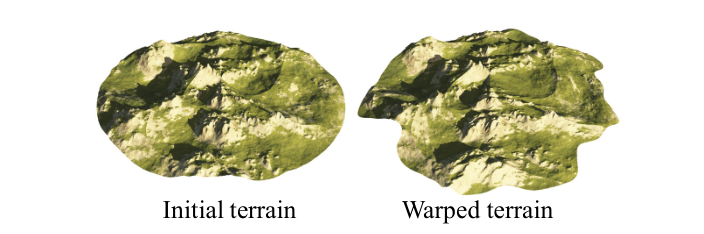
\includegraphics[width=.8\linewidth]{GGP15/warp_operator}
	\caption{This figure shows a deformed terrain using the warping operator.}
	\label{fig:warp_operator}
\end{figure}
\subsection{Rendering}
The paper proposes two different methods of rendering the tree structure. An advanced approach on Sphere Marching allows for high quality images at an interactive frame rate. The second algorithm uses adaptive quad tree tessellation with dynamic level of detail. The algorithm allows for multi resolution and crack-free terrain generation. Furthermore techniques like view frustum culling and distance based adaptive tessellation can be used to reduce computational costs. 

\section{Interactive physically based Fluid and Erosion Simulation}
The behaviour of water massively influences the look and features of a terrain. Depending on the timespawn, amount of water, ground composition and many more factors, hydraulic erosion creates a variety of different, but distinctive ground deformations, such as ripples, ridges, meanders, riverruns and valleys. 
This paper \cite{Neidhold:2005:IPB:2381356.2381361} presents an approach capable of creating such deformations in short amount of time, making it suitable for interactive visualization. The model represents terrain and water surfaces using height field, which is sampled onto a regular grid. A shallow water model is used to update the water surfaces and the fluid velocity field. 

\subsection{Water simulation}
This paper uses a simplified Navier-Stokes equation to simulate the water flow. The approach discards 3D-features like multiple water layers, vertical vortices and waves. this makes the equation less physically correct, but much faster to compute. The approach is based on a system of first order differential equations. This system describes the movement of material, in this case the amount of water at each cell, depending on velocity $\vec{v}$ and acceleration $\vec{a}$. Since this approach is dealing with complex erosion, the system uses am multidimensional material vector storing additional parameters like dissolved sediment.
$$\dot{\vec{v}} = \vec{a} -K_A \cdot \vec{v}=\frac{\vec{F}}{m} - K_A\cdot \vec{v}$$
$$K_A$$ describes the friction between the fluid and the terrain and can be manipulated for test purposes. 

\begin{figure}
	\centering
	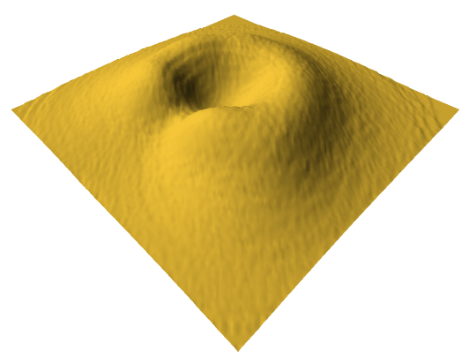
\includegraphics[width=\linewidth]{NWD05/hydraulic_errosion_a}
	\caption{Original model.}
	\label{fig:calc_acceleration}
\end{figure}

\begin{figure}
	\centering
	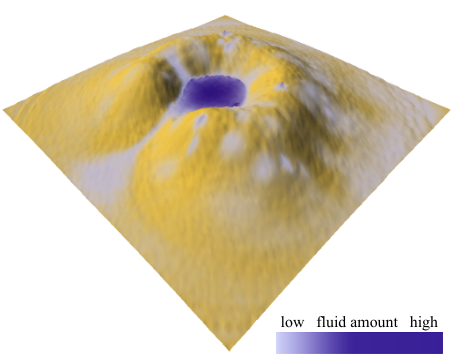
\includegraphics[width=\linewidth]{NWD05/hydraulic_errosion_b}
	\caption{Fluid simulation.}
	\label{fig:calc_acceleration}
\end{figure}

A vector field assumes that the particles movement is constant. In a common Newtonian Physic System objects are accelerated by the gravity. The direction of acceleration is the direction of the biggest tile angle $\alpha$ of the underlying height field. Therefore the acceleration force can be computed from the sinus of $\alpha$ times the gravitational constant g. The angle $\alpha$ is determined by the gradient $\nabla I(x,y)$ of the height field. 

At this point he acceleration direction is only defined in x and y direction. The acceleration vector $\vec{M}$ can be computed using the gradient $\nabla I(x,y)$: 
$$\vec{M} = (- \frac{\Delta I}{\Delta x}, - \frac{\Delta I}{\Delta y}, - \frac{\Delta I^2}{\Delta x^2}, - \frac{\Delta I^2}{\Delta y^2})^T$$
The acceleration vector can now be computed as follow: 
$$\vec{a}= \frac{|\vec{M}_z|}{|\vec{M}|} \cdot g \cdot \frac{\vec{M}}{|\vec{M}|}$$

$\vec{M}_z$ describes the acceleration direction direction along the z axis.

\begin{figure}[htb]
	\centering
	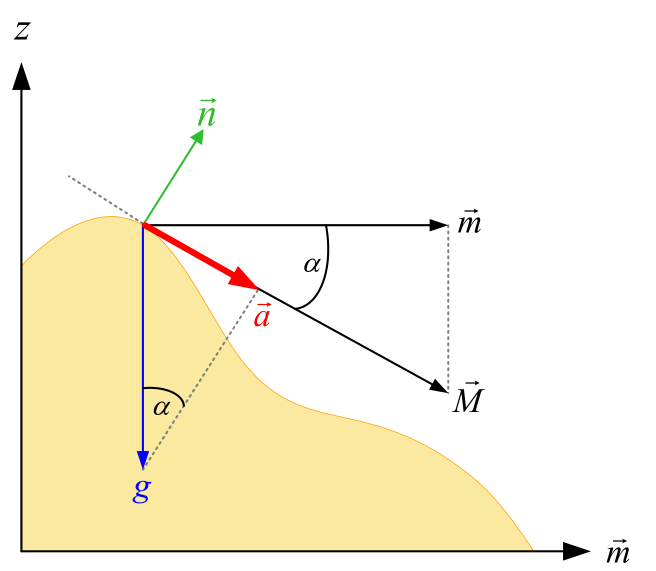
\includegraphics[width=.8\linewidth]{NWD05/acceleration}
	\caption{Calculation of acceleration.}
	\label{fig:calc_acceleration}
\end{figure}

\subsection{Hydraulic erosion function}
When water flows, soil, stones and other materials are dislocated and transported to lower regions. Whenever a part of material is moved to another grid cell by the simulation a hydraulic erosion function is used. It determines the amount of dissolved and deposited parts of material. The function uses the amount of transported fluit $\Delta F$ and the amount of sediment dissolved in this fluid $\Delta S$ as input. The function determines whether sediment can be deposited to or dissolved from the underlying cell. The function uses three major constants. 
\begin{itemize}
\item A \textbf{sediment capacity constant} $K_C$ determines how much of the underlying material can be dissolved per unit of water at a velocity of one. 
\item \textbf{The deposition constant} $K_D$ controls the rate at which soil is deposited at the target grid cell. 
\item The \textbf{dissolving constant} $K_S$ controls the dissolving rate of the underlying terrain into the fluid per simulation step.
\end{itemize}

The sediment capacity $c_S$ specifies the maximum amount of sediment that can be transported by the fluid $\Delta F$. $\Delta t$ scales the equation correctly at time steps unequal to one.  
$$ c_S = \frac{K_C}{\Delta t} \cdot \Delta F  \cdot |\vec{v}|
$$
If the amount of dissolved sediment $\Delta S$ exceeds the sediment capacity $c_S$, deposition is happening, otherwise the fluids capacity is not yet used fully, therefore more material is dissolved into the liquid. 

If $\Delta S > c_S$ deposit: 
$$
H = H + \frac{K_D}{\Delta t} \cdot ( \Delta S - c_S )
$$
$$
S = S + \Delta S - \frac{K_D}{\Delta t} \cdot (\Delta S - c_S)
$$
If $\Delta S <= c_S$ dissolve: 
$$
H = H + \frac{K_S}{\Delta t} \cdot ( \Delta S - c_S )
$$
$$
S = S + \Delta S - \frac{K_S}{\Delta t} \cdot (\Delta S - c_S)
$$

Both cases modify the height H of the terrain at the given cell. Depositing increases the height and decreases the sediment dissolved in the fluid, whilst dissolving decreases the height H and increases the sediment amount in the fluid. The material constants $K_D$, resp. $K_S$ additionally scale the equation for erosion of different materials. 

\begin{figure}
	\centering
	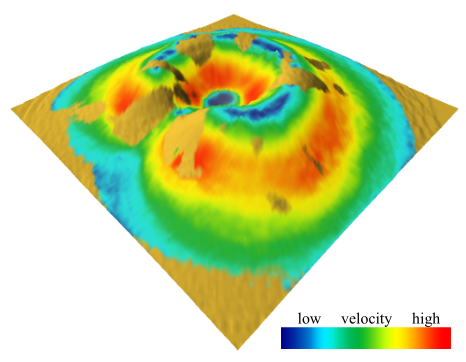
\includegraphics[width=\linewidth]{NWD05/hydraulic_errosion_c}
	\caption{Color-coded fluid velocity}
	\label{fig:calc_acceleration}
\end{figure}

\begin{figure}
	\centering
	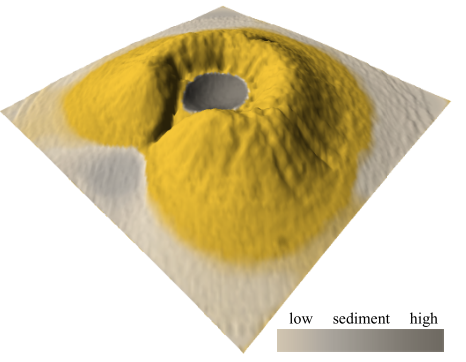
\includegraphics[width=\linewidth]{NWD05/hydraulic_errosion_d}
	\caption{Eroded terrain after 300 simulations steps with color-coded depositing}
	\label{fig:calc_acceleration}
\end{figure}
\section{Terrain Generation Using Procedural Models Based on Hydrology}
\label{sec:Hydrology}
Previously we introduced an approach that made use of local terrain features in various combinations to create terrains. This process was not procedural and heavily depended on the artists creativity to place and scale local features. In \cite{Genevaux:2013:TGU:2461912.2461996} a more modest approach is introduced, which generates a terrain procedurally around a given set of features, namely river networks.
 
\subsection{River Network Generation}
A river network can be interpreted as a graph, whose nodes act as either a spring, river mouth, or as a fork. 
The first step is to create a set of initial candidate nodes on the contour $\Gamma$, which act as river mouths. The user can additionally sketch some parts of the rivers. Initial nodes are placed on regularly jittered sample locations on the sketch. Each not is assigned a priority index, defining the overall appearance of the resulting river network hierarchy. 

\begin{figure}[htb]
	\centering
	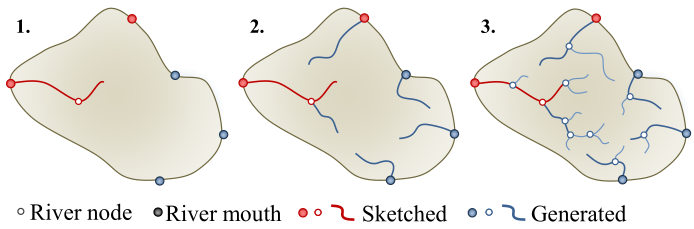
\includegraphics[width=\linewidth]{GGG13/river_network_sketch}
	\caption{Successive growing of the river graph. }
	\label{fig:river_network_sketch}
\end{figure}

For generating the network, the geometric graph $G$ is incrementally grown and elevated using a probabilistic approach. For each candidate node in $G$ the following steps are performed. 
\begin{enumerate}
	\item A \textit{Node selection}: choose a node $N$ from $G$ to which will be expanded.
	\item \textit{Node expansion}: expand the choosen node and perform geometric tests to verify its compatibility with the previouly created nodes. 
	\item The \textit{Node creation}: add the expanded node $N$ to $G$ 
\end{enumerate}

\subsubsection{Node selection}
The node that will be expanded is selected using a heuristic that takes into account the node elevation and its priority index. The combination of the two criteria allows a simultaneous creation of multiple networks competing for space. 
First we find the candidate node with the lowest elevation $z$. 
$\zeta $ is a parameter, that controls maximum range of elevation. Therefore we obtain a subset of admissible nodes, that are within the range of $[z, z + \zeta]$. From this set, the node with the highest priority index is chosen. if more than one node satisfies this criterion, the node with the lowest altitude will be chosen. 

Therefore the value of $\zeta$ directly influenced the appearance of the networks. If the decision is mainly based on the priority index (large $\zeta$), large networks are created. In contrast, if the elevation is pivotal, many local networks of similar sizes are created.

\begin{figure}[htb]
	\centering
	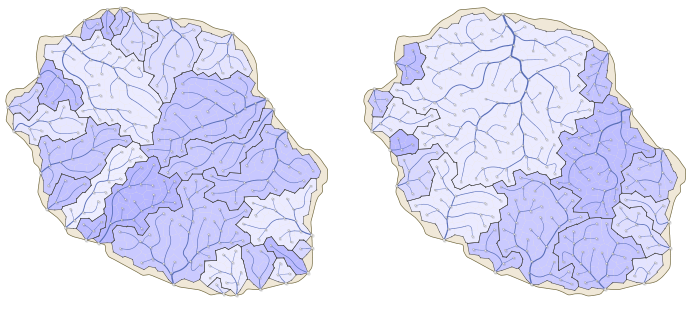
\includegraphics[width=\linewidth]{GGG13/drainage_system}
	\caption{Different networks are obtained from different $\zeta$ values. With $\zeta = 0$, we obtain networks of similar sizes. When using a high value $(\zeta = 20)$, one large network suppresses other networks. }
	\label{fig:river_network_sketch}
\end{figure}

\subsubsection{Node expansion}
To guarantee a consistent water flow, the elevation of a new node hast to be higher than its ancestors. This can either be achieved by using a river slope map. Such a map describes an intuitive way of how the network will expand. The probabilities $P_a, P_s, P_c$ for asymmetric branching, symmetric branching, or simple continuation without branching have to be predefined. 

To determine whether an expansion is valid, the system uses Horton-Strahler numbering. The Horton-Strahler number of a leaf  is $s$ = 1. An inner node inherits the maximum Horton-Strahler number from its children. If more than one children share this number, the Horton-Strahler number gets increased by 1.

For evaluation the tree is populated with the priority indices of the nodes. Using the probabilities  $P_a, P_s, P_c$ the type of the selected node is compared its possible new neighbour. Additionally the geometric properties of the graph are checked in order to prevent invalid nodes causing collisions and loops.  
\begin{figure}[htb]
	\centering
	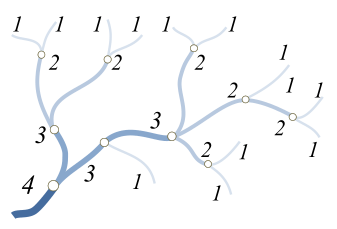
\includegraphics[width=0.5\linewidth]{GGG13/horton-strahler}
	\caption{Horton-Strahler numbering.}
	\label{fig:horton_strahler}
\end{figure}

\subsection{River Classification}
Once the river graph is build, the domain is divided into non overlapping cells, computed from the Voronoi diagram of node locations.  
The watershed of a cell $s$ is defined as the set of upstream connected cells and are associated with each water outlet of a cell. Its area is approximated by the sum of areas of cells connected to s. This is used to calculate the mean flow of the river. 

\begin{figure}[htb]
	\centering
	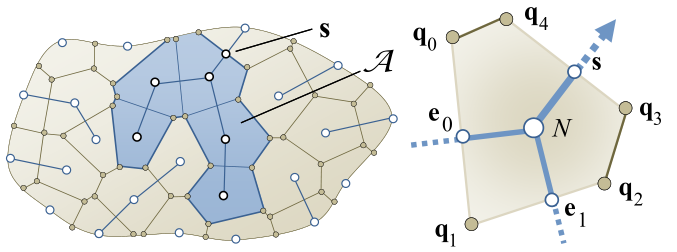
\includegraphics[width=\linewidth]{GGG13/voronoi_watershed}
	\caption{Example of watershed(blue) and a Voronoi cell.}
	\label{fig:voronoi_watershed}
\end{figure}

An edge of a Voronoi cell intersecting the river graph carry a connection to other river cells. Therefore the cannot be elevated. Edges that do not intersect the graph are used to compute the elevation of ridges between several streams. The points of this edge are called crest points. Each crest points is located at an equal distance $d$ from the centers $a, b, c$ of neighboring river nodes. Looking at figure \ref{fig:crest} the crest q should have a higher elevation than $a$, $b$ and $c$, insuring a continuous water flow. The elevation $q_z$ is computed as follows: 

$$q_z = max(a_z, b_z, c_z) + \lambda(q) \cdot d, \\ \lambda \in [0; 0.25]$$ 

$\lambda$ describes a slope magnitude function that describes if the terrain is mountainous. This terrain slope map can be set by the user or generated prodedurally. 
\begin{figure}[htb]
	\centering
	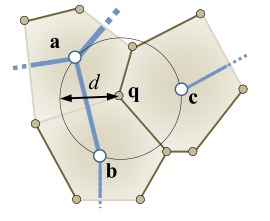
\includegraphics[width=\linewidth]{GGG13/crest}
	\caption{Calculation of the crest elevation.}
	\label{fig:crest}
\end{figure}

Each cell is assigned a class label, that corresponds to the type of river. Each class has a trajectory type and a digging profile of the riverbed. It includes geological composition of the riverbed. Each node is assigned such a label based on the river slope, and its proximity to the coast. 

\subsection{River Primitives Generation}
Each cell gets represented by a primitive. First all junctions are generated in a cell. The process starts by connecting two neighbouring water entries inside the cell. Incrementally all consecutive entries are added to the previous stream. Finally the stream is then connected to the water exist. The connection angle of two rivers is defined by the amount of water flow in the streams. Junctions of two rivers with the same size will cause a small junction angle, whereas a vastly difference in water flow will result in an almost perpendicular angle. 

\subsection{Terrain Model Generation}
Each river class has predefined profiles and a base trajectory of river flow. Using this information, the terrain primitives are generated with the same approach presented in section ~\ref{sec:tmffp}. This allows for additional terrain features and noise textures to be combined with the river flow, to create realistic looking terrains. 
\begin{figure}[htb]
	\centering
	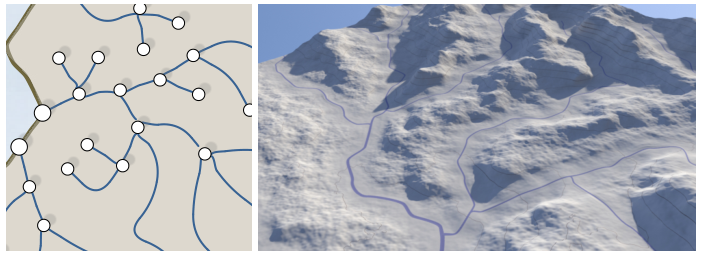
\includegraphics[width=\linewidth]{GGG13/valleys_and_rivers}
	\caption{Rivers and valleys created with a river graph.}
	\label{fig:valleys}
\end{figure}

\section{Real-time Animation of Sand-Water Interaction}
We all came across wet sand in one way or the other. Might is have been when building sandcastles as a child, or relaxing at the beach during a vacation. But modeling such a rather common phenomenon is much more difficult than one might expect.

\begin{figure}[htb]
	\centering
	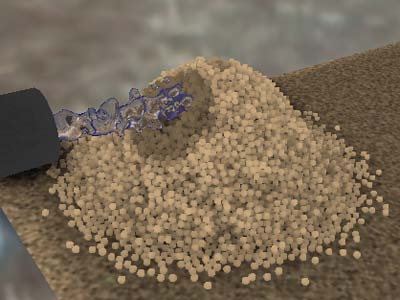
\includegraphics[width=\linewidth]{RSKN08/pileofsand.jpg}
	\caption{Calculation of sand, when water is added.}
	\label{fig:pileofsand}
\end{figure}

Although sand and beach environments are quite common in many commuter games, the physically correct simulation of sand-water interaction has only been approached recently. A very promising method was proposed by \cite{rungjiratananon2008real}. The approach is based on modeling every grain of sand as a separate particle. Each such particle as a specific "wetness" value assigned to them. This represents if we are dealing with dry, wet or "overwet" sand (see Figure \ref{fig:wetness} and \ref{fig:wetsandtypes}). Another crucial thing to take into account are the liquid bridges, which are formed between sand particles when fluids (water) are introduced.

\begin{figure}[htb]
	\centering
	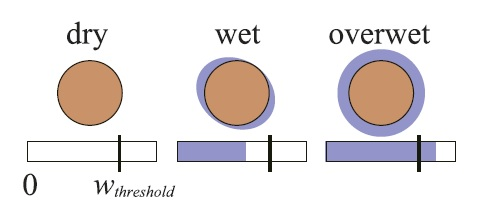
\includegraphics[width=\linewidth]{RSKN08/wetness.jpg}
	\caption{The different wetness levels of a (sand) particle.}
	\label{fig:wetness}
\end{figure}

\subsection{Two different models}
The two different models utilized here are Smoothed Particle Hydrodynamics (SPH) \cite{rungjiratananon2008real} and the Discrete Element Method (DEM) \cite{rungjiratananon2008real} (see Figure \ref{fig:domains} ).

\begin{figure}[htb]
	\centering
	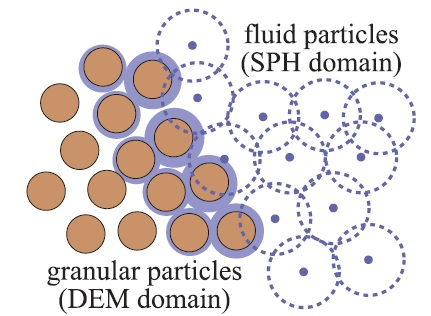
\includegraphics[width=\linewidth]{RSKN08/domains.jpg}
	\caption{Difference between DEM and SPH domain.}
	\label{fig:domains}
\end{figure}

While SPH is used to calculate forces within a particle, DEM helps calculation the attractive forces between multiple particles. If the 1st or the second model is used depends on the wetness value. exceeding a specific: If the wetness is high enough, liquid bridges are formed and therefore inter-particle forces have to be taken into account. Since those forces are quite string, gravity and moisture absorbed from the air are not considered to be part of the result and therefore not tackled in this approach.

\subsection{Performance and real-time usability}
Since every particle has to be treated completely separately resulting in a high amount of parallel computations, this is done on the GPU most efficiently. This vast number of calculations results in a "moderate" frame rate when trying to simulate more complex scenarios. The results from \cite{rungjiratananon2008real} where achieved with common Hardware from 2008, resulting in around 40 fps for 32k granular and 32k fluid particles, and drops down to 4 fps when using 33k granular and 64k fluid particles respectively.

\begin{figure}[htb]
	\centering
	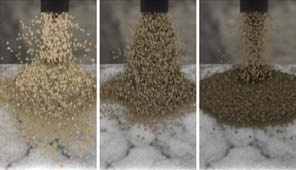
\includegraphics[width=\linewidth]{RSKN08/wetsandtypes.jpg}
	\caption{Illustration of the 3 differed wetness levels.}
	\label{fig:wetsandtypes}
\end{figure}
\section{Hydraulic Erosion Using Smoothed Particle Hydrodynamics}
In this publication \cite{krivstof2009hydraulic} a novel approach is presented, in which a physically based erosion system can be calculated in real-time. The Base concepts are quite the same as in the previously mentioned publication, but is the title already reveals the already know SPH is used as underlining base model here.

\begin{figure}[htb]
	\centering
	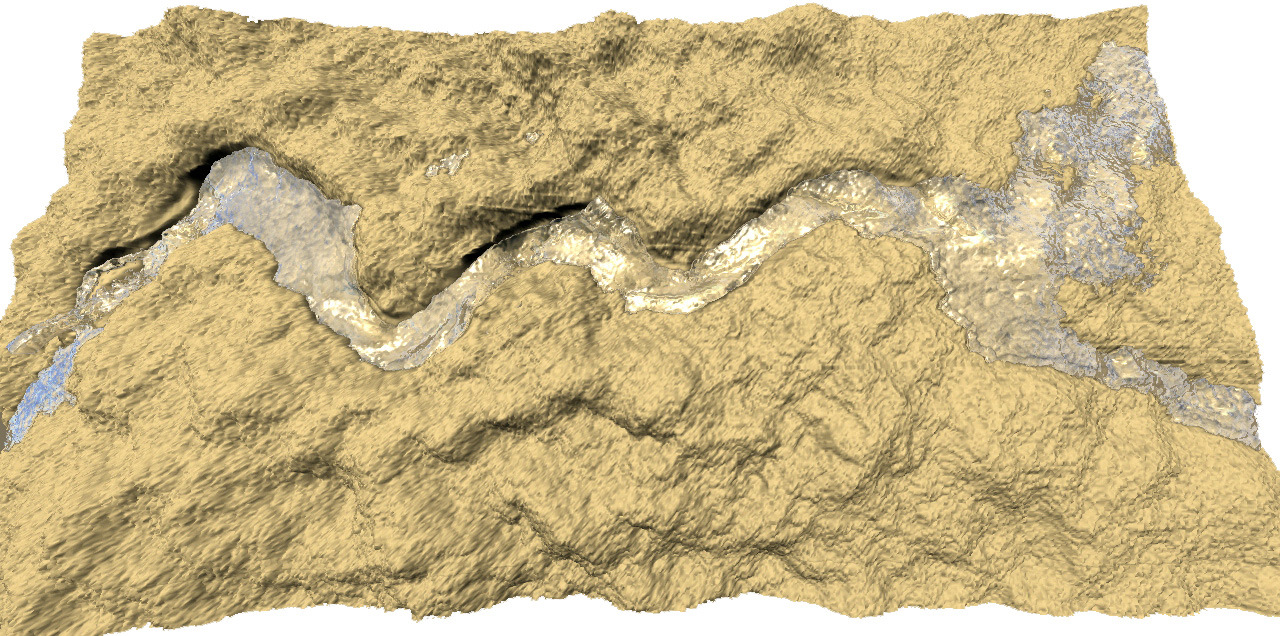
\includegraphics[width=\linewidth]{KBKS09/illustration1.jpg}
	\caption{Rendering of the path of a river in soil.}
	\label{fig:illustration1}
\end{figure}


\begin{figure}[htb]
	\centering
	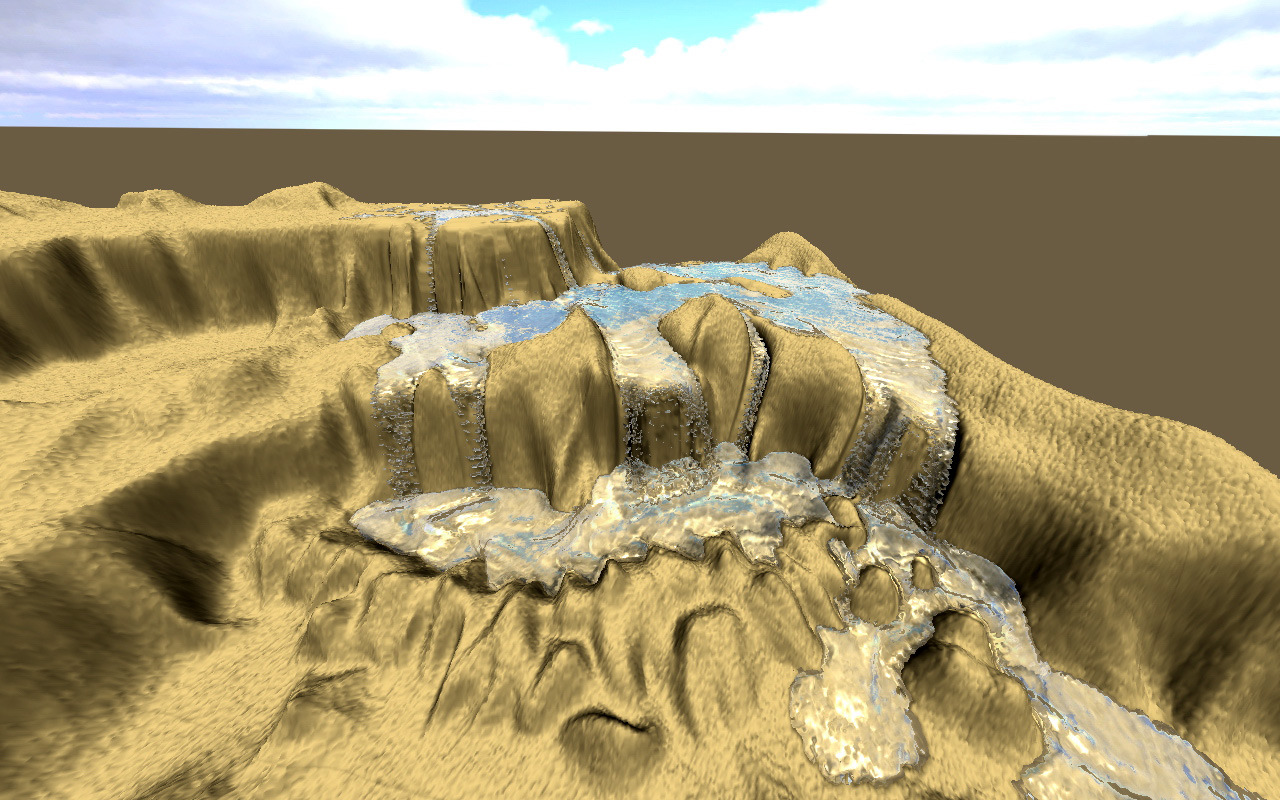
\includegraphics[width=\linewidth]{KBKS09/illustration2.jpg}
	\caption{Rendering of terrain erosion through water.}
	\label{fig:illustration2}
\end{figure}

\subsection{Two different approaches}
An important distinction is mode between two different calculation approaches:

\subsubsection{The Eulerian model}
The Eulerian models focuses on hydraulic erosion effects and therefore use a static grid of points. A full scale 3D calculation on approach for erosion calculation is almost impossible to be done in real-time. Most used methods therefore rely on "2.5D" methods, which combine purely surface- / plane-based models with parts of a full 3D approach.

\subsubsection{The Lagrangian model}
Lagrangian models are based on SPH and calculate their results on particle basis. Due to that fact, these methods are much more scalable. Since everything is calculated on particle basis, this approach yields better more exact results in areas, with a high density of particles.

Since there are a lot of necessary calculations to be done which increase linearly with the number of particles, a purely 3D calculation model is rarely used here. As with the Eulerian approach, a combination of calculations on 2D and 3D basis is used. Although this method was not exactly designed with real-time rendering in mind, the resulting "2.5D" approach yields relatively good results while still remaining reducing the time needed to the calculations drastically.

Since in SPH based approaches all calculations are particle-based, many physical (side-)effects can quite easily be implemented. The basic sediment transport can be calculated using widely known formulas \cite{krivstof2009hydraulic}. In addition to that, in a Donor-Acceptor Scheme (see Figure \ref{fig:donoracceptor}) is used here, which takes interaction between particles along their velocity, as well as gravity into account \cite{krivstof2009hydraulic}.

\begin{figure}[htb]
	\centering
	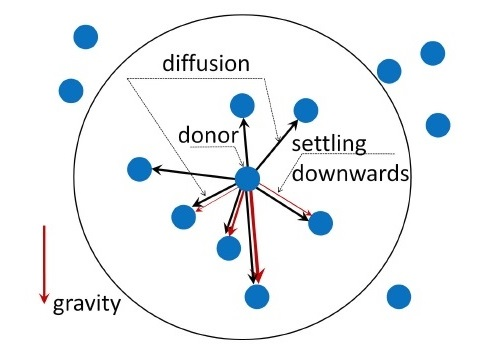
\includegraphics[width=\linewidth]{KBKS09/donoracceptor.jpg}
	\caption{The Donor-Acceptor Scheme.}
	\label{fig:donoracceptor}
\end{figure}

An important concept here are the so called "boundary particles", which also play an important role in the aspect of Terrain Modification as it can be seen in Figure \ref{fig:illustration1} and \ref{fig:illustration2}. Those particles basically are the "communication" between the fluid particles (SPH) and the soil where the boundary particles are placed. In the first iteration the erosion and deposition are calculated, and in the second step / iteration the actual deformation of the terrain itself is performed (see Figure \ref{fig:boundary2}). 

\begin{figure}[htb]
	\centering
	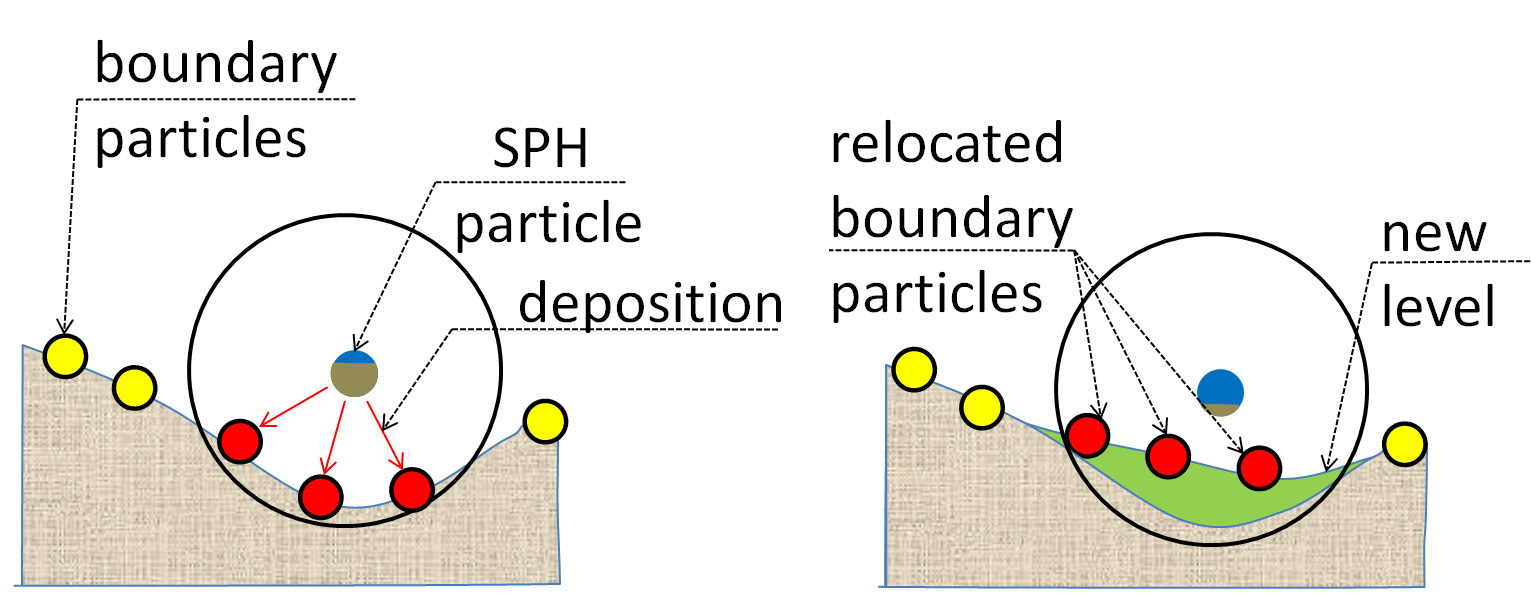
\includegraphics[width=\linewidth]{KBKS09/boundary2.jpg}
	\caption{SPH boundary particle relocation.}
	\label{fig:boundary2}
\end{figure}

\subsection{Performance}
Since this approach was, as mentioned before, not designed with any real-time applications in mind, the underlying publication does not provide us with comparable frames-per-seconds values or something like that. What the authors do present, are vales of how long a single calculation step takes for a certain amount of particles and for every discussed method.

It has to be kept in mind, that those number represent just the time needed for the actual calculation. Therefore they can not simple be converted to fps since there would of cause be some overhead in computing the actual visualisation in addition to the calculations of the underlying model itself. But for the sake of comparison, we did translate those number into rough fps-estimations which can easily be done by taking the reciprocal value of the needed time in seconds needed. In doing so, we quickly realize that this approach is (at least with the used hardware) far from real-time capable.

The utilized hardware was quite common at that time (2008): a Quad Core CPU and a NVIDIA 8800 GT. The average frames per seconds are about 3.3 for 90k particles and around 2.2 for 136k particles. The specific hardware components and complete results can be found in \cite{krivstof2009hydraulic}.




\section{Layered Data Representation for Visual Simulation of Terrain Erosion}

\cite{marechal2010heat} - !!! RAW TEXT !!!
%DEL: \cite{cordonnier2016large}

This Paper focuses on introducing a completely new data-structure to store terrain-information which makes calculations much easier to perform. The two opposing conventional methods of storing and handling such data have already been explained before:
- Voxel Representations which allow for accurate calculations but have very high memory demands
- Representations of the just the terrain-surface with hightfield(s) where precision and accuracy is sacrificed in order to gain space and reduce computing requirements.

Many different techniques have already been discussed here and many more have been developed. Some of the most common ones include fractal interpolation to generate hills and water streams (---) or blending some elaborate noise functions to generate visually plausible results (---). But all of there approaches have one thing in common: while the accuracy of true 3D Voxel representation is often approximated quite well, is is never truly reached with those techniques.
To overcome this limitation and enable very accurate calculations, which are meant to be used in physical simulations rather than in realtime environments, the authors generated a mixed data-structure combining Voxel and hight filed representations.

\subsection{A novel datastructure}
Since in many areas of a given terrain full Voxel data would be "waste  of data" \cite{marechal2010heat} since the represented layers are usually quite thick, one can reduce the needed space in some areas. This approach used in this paper is to use a 2D array of 1D arrays as representation of terrain. This can be  imaged as a core sample, where each layer in itself is supposed to be constant (or rather is's parameters are). The hight of the position can easily derived from a "core samples" hight and it's index.
The big advantage of this kind of data structure is it’s easy and fast traversal with a much smaller effort (and thus higher speed) as it would be the case for a conventional pure-Voxel approach. Another positive side effect of storing data this was is that the data structure also allows for zero-density layers. This way also caves and even material falling from the ceiling of those caves (along the inverted surface gradient) can be captured and therefore be used to perform calculations. That way erosion can not only be performed on the terrain-surface, but also in all sub-surface holes existing or developing in the terrain \cite{marechal2010heat}.

\subsection{Efficiency}
The calculations to test the efficiency of the newly introduced data structure were performed on an Intel III with 500MHz, and a freeware tool was used to generate simple visualizations. The calculation of 100 erosion steps on a 1024x1024 element grid with 5 layers took 239 minutes for example. Other calculation taking much longer were also tested, including ones, that could not be done with relying on only hight filed data. The full and exact specs and results can be found in the original paper \cite{marechal2010heat}.
\section{Interactive physically based Fluid and Erosion Simulation}
...



\section{Heat Transfer Simulation for Modeling Realistic Winter Sceneries}

text \cite{benes2001layered}.
!!! RAW TEXT !!!

While many of the previously presented papers strictly deal with erosion in combination with evaporation and seminentation alone, the temperature is mostly assumed to be constant. In some simpler cases it is not take into account at all. In paper presented in this chapter, exactly that often „overlooked“ topic becomes the primary focus of the calculations.

To allow more complex thermal calculation for simulating a natural environment, one needs to take a lot of different influences and physical processes into account. The existing methods prior to this paper primarily rely on one of those three approaches for calculating winter scenarios for example:
\begin{itemize}
	\item Particle based snow accumulation
	\item Surface displacement methods
	\item Ice growth
\end{itemize}

The name of these methods basically already implies what they fundamentally do:
The particle based accumulation methods evaluate the trajectory of snowflakes (blown by the wind) colliding with the surface (). In an alternative approach the stochastically generated snowflakes are „shot up in the sky“ and the calculations are done recursively. Non of these methods are truly physics-based and both either include solving Navier-Stokes () or the Bolzmann equations (). The only physics based system mentioned, works on basis of vortex fields and incorporates melting snow, but leaves the weather completely aside.

The surface displacement methods basically only calculate the hight of the accumulated snow falling on a specific spot. This can easily be done by using the depth buffer () or through dissipating calculated ambient occlusion with illumination (). Another very efficient variant of this approach is done by using hight span maps and heavily relies on a statistical model for snow accumulation derived from observations in nature ().

Calculating ice growth is not used so widely. Some methods simulate ice crystal formation over objects by using a phase field method (). Another more sophisticated hybrid-approach combines those phase filed methods with fluid simulation and procedural defused limited aggregation ().

\subsection{The newly proposed approach}
Like many other methods, this one also relies on a voxel grid. Like for so many other authors before mentioned, the challenge is to find the right balance between a high-resolution grid which is able to capture small details, and a large scale grid which requires less memory and computational effort.

Here this problem is handled by evaluating the evolution of temperature of every voxel, taking into account changing weather and environmental conditions (and therefore temperate) over time. After that a hightfield is generated for the surface representation, from the hight of snow stored in the according voxels ().

The data structure used for the calculation consists of a grid of voxels, where for each voxel one (or two) materials, the temperature and the percentage of solid material are stored along with energy exchange over time. Since some voxels can contain two materials at once (e.g. ice and water or snow and air), these voxels need to be evaluated more carefully. Phase transitions are more likely to occur in those „mixed“ voxels than in any other one.

\subsection{The calculation process}
In the calculation technique itself its rather complicated and it will only by presented as an overview here. Due to it’s highly physically-based background the results are very accurate, but not meant to be used for realtime calculations.

The necessary calculations for this approach is performed in four different steps:
\begin{enumerate}
	\item Compute environment parameters
	\item Simulate snowfall and accumulation
	\item Compute thermal (and energy) transfer between voxels
	\item Computer phase-change for affected voxels
\end{enumerate}

These five materials are key to all calculations performed here: Rock, Ice, Water, Snow, Air. Every material has it’s own constraints and attributes. Some of this attributes are mass density, specific heat capacity, thermal conductivity, emissivity, melting temperature, etc.

In addition to the materials itself, there are a number of global factors and attributes needed for the calculation, which are defined in the environmental model. This model defines the development and change of weather over time. Weather itself is defined as air temperature, dev point, the amount of snowfall, the cloud cover as well as information about day- and night-cycles.

All thermal transfers happening in the simulation can be categorized as one of the following types:
\begin{itemize}
	\item Conduction is the heat-transfer between to media in contact
	\item Convection takes place within fluid materials and on the boundaries to solid materials
	\item Radiation is defined as energy emitted as (electro-magnetic) waves from a surface
\end{itemize}

Without going too much into detail here it can again be stated that these calculations are based on several physics-equations and take a lot of detailed factors and influences as well as properties into account. For example can the warming up of a surface from the energy (heat) impact through sun-rays not only be assumed to be constant. In this computational model the temperature of the sky itself is needed to get an result. This temperature does depend on the temperature of the air at this time, and the dew point temperature. In addition to that the degree of the sundays hitting the surface is evaluated. If the sky is not assumed to be cloudless, the amount of vapor in the air (which is decreasing with the dew point temperature) has also to be taken into account. After that, the actual filtering of the sun-rays through one or more clouds can be applied. Another good example is the calculation of indirect heat, which is reflected from nearby surfaces and can effect snow-melding in the mountains in nature for example.

For the phase changes from one material to another, a fusion temperature is defined. If this temperature is reached, the (partial of complete) transition of this voxel is performed. Since some aspects go ever further into detail than this paper already does, things like the dynamics of flowing water is approximated in the calculations. This would have to be done in addition to computing the absorbtion and evaporation of water through solid ground (rock) and therefor distinguishing between dry and wet rocks. Also the possibility of flowing water freezing during movement due to slow flowing speeds and low temperatures of the ground, is not take into account here. Another interesting physical phenomenon included in this model’s calculations are different temperatures within a lake or even a puddle of water. Since the weight of water changes a little with its temperature, and the sun generally warms the upper layer of a lake more than the lower parts of it, a lake or pond can come times be decided into more than one different temperature zones.
For generating Snow on a surface-level or freezing water resulting in ice, a more approximated technique is used. Snow on the surface is simple represented by a textured hight field, which is obtained by the elevation of the vertex grid at that point. For freezing water inside a like, two hight fields are generated: one for the upper and one for the lower surface of the developing ice. The the separation of those, the thickness of the ice-layer can be controlled.

\subsection{Performance}
As is can easily be derived from the complexity of the calculations done in this approach, this technique was never meant to be performed in realtime. Although the time step can be set relatively large, since thermal effects occur much slower than many other natural phenomena, the time needed for the calculations is still quite high.

Nevertheless the paper include one relatively simple example of a landscape simulation, along with the time it took to compute. The implementation used was written in C++ and run on an Intel Dual-Core processor with 3GHz and with 3GB RAM. On this hardware the calculation for a nine day weather model on a grid of 3.2 million voxels tool about 5 hours ().

!!! RAW TEXT !!!
blaa\cite{cordonnier2016large}
blaa\cite{benes2001layered}


%------------------------ REFERENCES ------------------------%

\bibliographystyle{eg-alpha-doi}
\bibliography{references}


\end{document}

